\documentclass[conference]{IEEEtran}
\usepackage{cite}  
\usepackage{graphicx}  
\usepackage{paralist} 
\usepackage{tabularx}    
\usepackage{url}       
\usepackage{balance}       
\usepackage{multirow}     
\usepackage{multicol}       
\usepackage[TABBOTCAP]{subfigure} 
\usepackage[pdftex]{graphicx}
\DeclareGraphicsExtensions{.jpg,.JPG,.png,.pdf,.eps}
\graphicspath{{img/}}    

\usepackage{amssymb}
\usepackage{ifthen}

\makeatletter

% this  is a easy way to comment out more lines ...

\newcommand{\COMMENT}[1]{}

% this  is a easy way to add and highlight new text  ...
% just comment in/out the \tnew macro ..

\newcommand{\tnew}[1]{{\bf { #1 }} }
%\newcommand{\tnew}[1]{{ { #1 }} }

% math and theorem definition

\newcommand{\ndef}{\stackrel{\rm def}{=}}

% this is used for draft only

%\renewcommand{\baselinestretch}{2}

% just to number pages in the draft

\pagenumbering{arabic}

% nothing i.e., no-numbering final and camera ready

%\pagestyle{empty}


\newboolean{showcomments}


\setboolean{showcomments}{true}


\ifthenelse{\boolean{showcomments}}
  {\newcommand{\nb}[2]{
    \fbox{\bfseries\sffamily\scriptsize#1}
    {\sf\small$\blacktriangleright$\textit{#2}$\blacktriangleleft$}
   }
   \newcommand{\cvsversion}{\emph{\scriptsize$-$Id: macro.tex,v 1.9 2005/12/09 22:38:33 giulio Exp $}}
  }
  {\newcommand{\nb}[2]{}
   \newcommand{\cvsversion}{}
  }



\newcommand\ROCCO[1]{\nb{ROCCO}{#1}}
\newcommand\MAX[1]{\nb{MAX}{#1}}
\newcommand\SEBASTIANO[1]{\nb{SEBASTIANO}{#1}}
\newcommand\MB[1]{\nb{MARTIN}{#1}}
\newcommand\GERARDO[1]{\nb{GERARDO}{#1}}

\newcommand\NEW[1]{\nb{NEW}{#1}}




                                           
                   
\begin{document}                             
                       
\title{Finding UUX Issues in User Reviews}
\author{\IEEEauthorblockN{  
E. Bakiu,
E. Guzman  
} 
\IEEEauthorblockA{Technische Universit\"at M\"unchen,
Garching, Germany} 
elsabakiu@gmail.com, emitza.guzman@mytum.de
}        
 
\newcommand{\etal}[0]{{{et al.}\ }}
\newcommand{\ie}[0]{{{i.e.}\ }} 
\maketitle
 
\begin{abstract}

%\boldmath 

\noindent
Usability and User Experience (UUX) play an increasingly significant role in the success of software products. There exist an extensive number of UUX evaluation methods. However, these methods are expensive in terms of time and human resources. Additionally, they capture the interaction of users with the system for a short time, in a non-natural environment. Users express their opinion about software products on review sites, social media platforms and blogs. They write detailed reviews of products, usually after a long time of interacting with them, while solving their actual problems. These reviews are not just summary assessments or recommendations, but also self-reports of the user's experience. Research shows that 49\% of the sentences extracted from user reviews contain UUX information.  However, due to the broad amount of reviews and their lack of  structure, it would be very inefficient to manually analyze them and extract relevant information. This underlines the clear need for an automated solution.

\noindent
In this thesis we propose an approach to automatically evaluate UUX information present in user reviews through the following steps: (a) extract usability and user experience information from user reviews using machine learning techniques, (b) evaluate the sentiment of each review sentence using sentiment analysis and (c) visualize the results in different perspectives to aid the detection of UUX problems. We achieved 68\% accuracy in detecting the presence of UUX information in review sentences and 71\% accuracy in predicting the sentences sentiment. The visualization component is introduced to illustrate the potential usage scenarios of the approach, however, it is in an early stage of development. 

\noindent
The proposed approach provides a quick UUX assessment method that allows a continuous evaluation process, incorporating user feedback over time and capturing aspects that are not captured by standard UUX evaluation methods such as spontaneity of opinions.

\end{abstract}

% no keywords
         
\IEEEpeerreviewmaketitle  
      
\section{Introduction}  
\label{sec:intro}   
Software quality is an important aspect of the software development process, and its absence might result in serious consequences such as financial and reputation loss \cite{Hussain2013}.
Software quality can be measured through conformance to functional requirements and other non-functional specifications defined by user needs\cite{Chattopadhyay2013}. Non-functional or quality requirements like usability, reliability, performance and supportability are factors which lead to a successful project \cite{Bayraktaroglu2009}. Various studies \cite{Lizano2013}, \cite{ Chattopadhyay2013} have highlighted the importance of software usability and in general of user experience as factors for promoting software success. 
Both, good usability and user experience (UUX), rely on user feedback through evalu- ation rather than simply trusting the experience and expertise of the designer \cite{Quesenbery2001}.
There exists an extensive number of UUX evaluation methods, however, these methods are expensive in terms of time and human resources.  They usually consist in getting feedback from the user through observations or direct interviews, in a non-natural environment. Furthermore, the interaction is captured only for a short time, making it difficult to evaluate dimensions of usability such as learnability or memorablity. Therefore, there is a need for alternative UUX evaluation methods that can address these vulnerabilities. 
User reviews offer great potential in addressing the limitations of the classical UUX evaluation methods. Users express their opinion and sentiment about software products in review sites, social media platforms and blogs. They write detailed reviews of products, usually after a long time of interacting with them, while solving their actual problems. In addition, these reviews are not just summary assessments or recommendations, but also self-reports of their experiences as users. Research shows that user feedback contains a considerable amount of UUX information. Hedegaard and Simonsen \cite{Hedegaard2013} found that 49\% of the sentences extracted from user reviews contain UUX information. However, due to the broad amount of reviews and their lack of  structure, it would be very inefficient to manually analyze them and extract relevant information. This underlines the clear need for an automated solution.
We must note though that the potential usefulness of online reviews has some important caveats, compared to laboratory usability studies. 
Obviously, the software must already be on the market to be evaluated publicly.
Further, the reviews contain very few details about the reviewer (e.g., gender, age or preferences) or could even be fake.
This means that the evaluation of UUX by analyzing user reviews cannot be a replacement for the existing methods, rather than an addition to address their limitations and to provide useful information that facilitates the process of software evolution. 
      
\section{Approach}     
\label{sec:approach} 
\subsection{Approach Overview}

In this work we propose an automated approach for evaluating the UUX of software products by analyzing user reviews.
For the purpose of this work, a review is a piece of text detailing positive and negative aspects of a product, an overall assessment (rating) and recommendations for potential buyers, written by a user of the product. We concentrate on reviews written in dedicated websites, for example: Epinions \cite{Epinions},  Amazon \cite{Amazon}, US App Store \cite{AppStore} and Google Play \cite{GooglePlay}.  Figure \ref{fig:introduction_review_epinions} shows an example of a review extracted from the Epinions website.
 		\begin{figure}[ht]
		\raggedleft
  			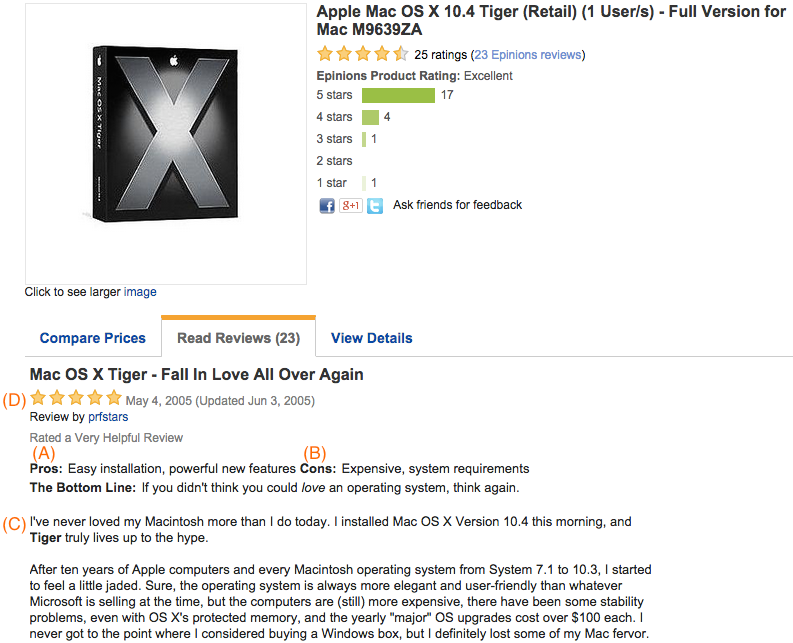
\includegraphics[width=0.4\textwidth]{img/introduction_review_epinions.png}
			\caption{Review example extracted from  Epinions website (28 January 2015). It details: (A) Positive aspects of the product, (B) Negative aspects of the product, (C) A general comment, (D) Overall assessment (rating).}
			\label{fig:introduction_review_epinions}
		\end{figure}

In this work, we propose a solution based on Natural Language Processing (NLP) techniques. NLP is a field of computer science, artificial intelligence, and linguistics concerned with the interactions between computers and human natural languages \cite{Bird2009}. One of the main applications of NLP involves natural language understanding, that is, enabling computers to derive meaning from human or natural language input.  This is our focus as our approach revolves around the analysis of written online reviews collected from dedicated review websites.  Specifically, we use machine learning techniques for UUX classification and sentiment analysis for determining the sentiment expressed in user reviews with regard to the product in general, or to features in particular. Fig \ref{fig:introduction_high_level_overall_approach_overview} depicts an overview our approach. 

		\begin{figure}[ht]
		\centering
  			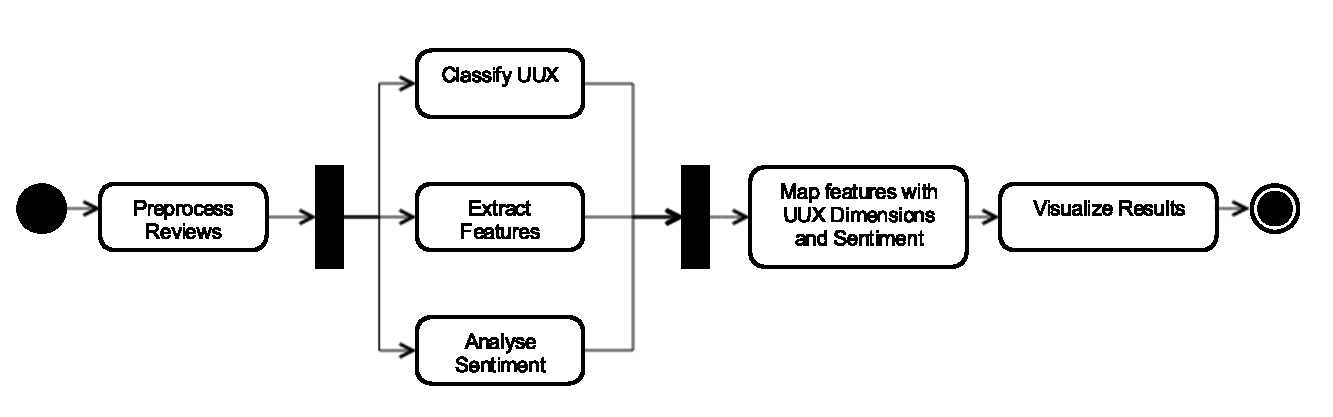
\includegraphics[width=0.4\textwidth]{img/introduction_acitvitydiagram_overallapproach.pdf}
			\caption{Overview of the approach (UML activity diagram).}
			\label{fig:introduction_high_level_overall_approach_overview}
		\end{figure}

One purpose of our approach is to provide an overall assessment of the sentiment of each UUX dimension, aggregated for the product in general, or fine-grained for each feature of the product. 
A UUX dimension can be a specific aspect, viewpoint, or phenomena within UUX (e.g., $Memorability$, $Satisfaction$, $Errors/Effectiveness$). A feature can be a description of specific software functionality (e.g., uploading files, sharing a link), a specific user interface (e.g., configuration screen, pdf viewer), a general quality of the software (e.g., price, privacy), as well as specific technical characteristics (e.g., encryption technology, multi-device syncing) \cite{Guzman2015}.
Our approach focuses on extraction of information from individual sentences, rather than entire reviews. As a review may incorporate both good and bad experiences relating to many different dimensions of UUX, a sentence-based bottom-up approach will yield more precise information about the ``typical" vocabulary associated to specific dimensions of UUX. By identifying the sentences that contain UUX information, we help the developers and UUX experts to filter the reviews by relevance and present only the most informative ones. 
Therefore, they can efficiently identify good and bad practices and gain insights on how to improve the product based on the users feedback.

\subsection{UUX Classification}

Initially, we construct a machine learning classifier that discriminates among dimensions based on words, or other features of the text that are automatically computed during the training of the classifier. The classifier automatically tags a sentence with the UUX dimensions it pertains to. This tagging task may be viewed as a set of binary classification tasks: for each dimension and each sentence, define whether the sentence relates to that dimension. 

For each UUX dimension, a binary machine learning classifier was trained and evaluated. Initially, the sentences were preprocessed, the data was split into five folds for performing cross-fold validation and then used for training the classifier. The feature vectors were weighted and ranked to discard the worst discriminating features. Finally, the SVM classifier was trained and standard performance measures were calculated.

\subsection{Sentiment Analysis}

The sentences containing UUX information are further analyzed and the expressed sentiment is detected. Similarly to the UUX classification, we use a machine learning classifier that categorizes each sentence as positive, neutral or negative. The approach is based on the hypothesis that people use specific words or phrases to express specific sentiments. Through the machine learning approach, the system can identify these 'keywords' and heavily rely on them for text classification. Furthermore, the system can learn how word phrases (e.g., bigrams) or punctuation are used to express specific sentiments.An unconventional step we took was negation handling. Hogenboom et al. \cite{Hogenboom2011} show that accounting for negation when analyzing sentiment in natural language texts helps improving the performance of classifying unseen natural language text as carrying either positive or negative sentiment. These results were also confirmed by our study. 

\subsection{Feature Extraction}

However, through the sentence level sentiment analysis we cannot understand what exactly users like or dislike about a product. User reviews not only express the overall sentiment about a specific product (e.g., ``This is a great  app"), but also sentiments related to its specific features, such as the functionality, performance, user interface, price etc. Subsequently, a review may convey opposing sentiments (e.g., ``Its performance is ideal, I wish I could say the same about the price") or objective information (e.g., ``You can adjust the volume, including normalizing all audio") for different features of a product.
Furthermore, the need for a fine grained analysis applies also to the UUX information. Users write their opinion about a product in general, however they can have different and even contradictory opinions about specific features of the product. 

\subsection{Merging of Classification, SA and Feature Extraction}


We perform a fine grained, feature level analysis as follows. Initially, the features are extracted and the feature sentiment is calculated as an average of the sentiment of the sentences that pertain to that particular feature. Similarly, the feature is mapped to all the UUX dimensions identified in sentences were the feature is present. For example, the sentence ``Still, it's a fun single player campaign, and a wonderful multiplayer experience"  is tagged by the UUX classifier with the following UXX dimensions: \textit{Hedonic, Pleasure, Affect/Emotion, Enjoyment/Fun}. The sentence level sentiment classifier tags the sentence as positive (fun, wonderful experience). The feature extraction process results in two features:  single-player campaign and multiplayer campaign. Finally, the two features are mapped with the sentence's UUX dimensions and sentiment as shown in Figure \ref{tab:example_results_approach}.

\begin{table}
\centering
\caption{The results of the approach for an example sentence: ``Still, it's a fun single player campaign, and a wonderful multiplayer experience".}
\label{tab:example_results_approach}
	\begin{tabularx}{\linewidth}{| p{4cm}|X| p{1.9cm}|}
	\hline
	\textbf{Features}&\textbf{UUX Dimensions}&\textbf{Sentiment}\\
	\hline
	Single-player Campaign&Hedonic, Pleasure, Affect/Emotion, Enjoyment/Fun&Positive\\
	\hline
	Multiplayer Campaign&Hedonic, Pleasure, Affect/Emotion, Enjoyment/Fun&Positive\\
	\hline
\end{tabularx}
\end{table}


\subsection{Visualization}

In the following paragraphs we introduce potential usage scenarios of the approach. 
Each usage scenario is supported by a visualization of the results (a report) that highlights specific aspects of the extracted information. The usefulness to the users, potentially developers and UUX experts (practitioners and researchers), is discussed for each usage scenario. 

In our main scenario, the user of the system gets an overview of the UUX sentiment on the most popular features of the system. The average sentiment of each UUX dimension across features and vice versa is visualized. In addition some of the most informative reviews for each UUX-feature pair are shown. These reviews are selected in such way that uniform distribution of review sentiment and rating is ensured.
Furthermore, users can search for particular features they are interested in and obtain the corresponding sentiment, the fine-grained sentiment for each UUX dimension and its most relevant reviews. Figure \ref{fig:introduction_scenario1} illustrates this scenario.
The purpose of this report is to provide a general overview of the sentiment of UUX dimensions across the most popular features. The users can easily identify the most 'problematic' features or UUX dimensions and further inspect them in the detailed reports described in the following paragraphs.


		\begin{figure}[ht]
		\raggedleft
  			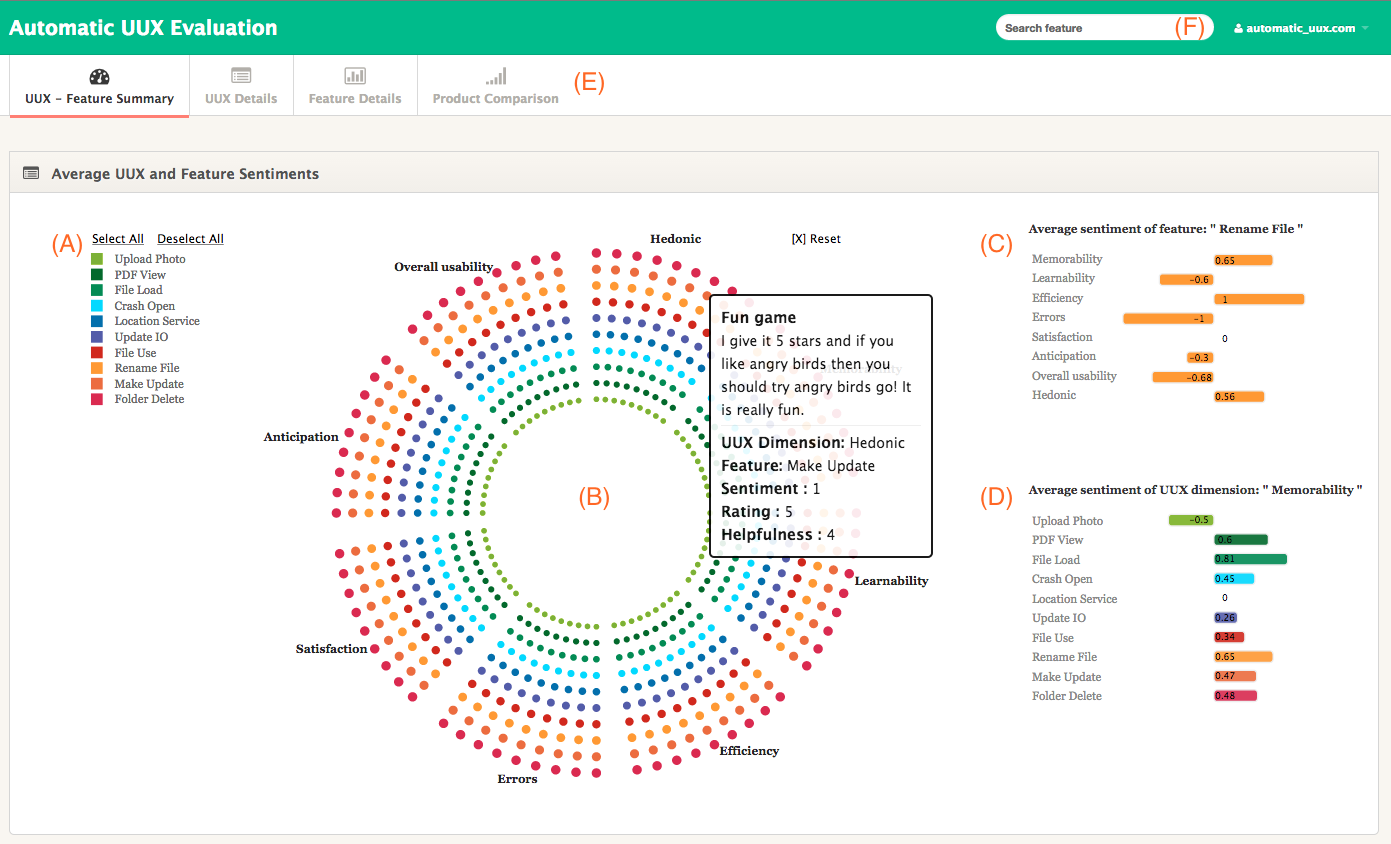
\includegraphics[width=0.4\textwidth]{img/introduction_scenario1.png}
			\caption{Feature-UUX overview. The following information is depicted in the view: (A) Most popular features (or the features the user has searched for), (B) Examples of some of the most relevant reviews for each UUX dimension-feature pair, (C) Average of the selected feature for each UUX dimension, (D) Average of the selected UUX dimension for each feature, (E) Navigation menu, (F) Search field to query features.}
			\label{fig:introduction_scenario1}
		\end{figure}

Another potential scenario is a fine-grained analysis of UUX.The average sentiments and the total number of reviews pertaining to each UUX dimension are depicted. The user can select a specific UUX dimension of interest and inspect the relevant user reviews over time, categorized based on the sentiment and rating. In addition, several statistics such as total number of reviews per sentiment level and average sentiment are shown (see Figure \ref{fig:introduction_scenario2}).
Initially, the visualized information is an aggregation over all features of the product. However, users can query for specific features they are interested in. 
A similar report would provide detailed information about the features of the product. The overall sentiment of the features or the sentiment with regard to specific UUX dimensions can be visualized. This report can be valuable especially to the development team by helping them identifying the most and least popular features and take decisions on how to improve them during software evolution.

		\begin{figure}[ht]
		\raggedleft
  			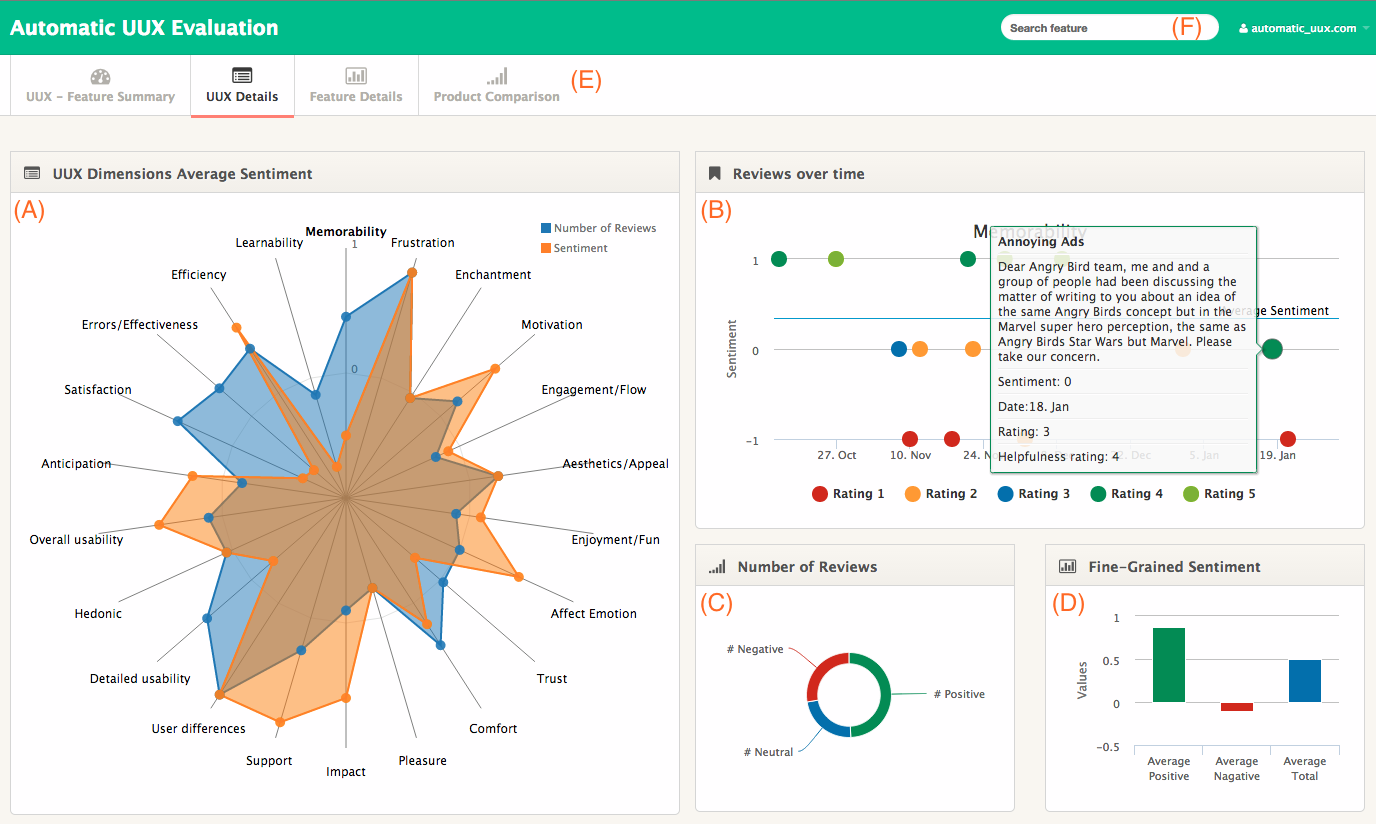
\includegraphics[width=0.4\textwidth]{img/introduction_scenario2.png}
			\caption{UUX Detailed View. The following information is depicted in the view: (A) Number of relevant reviews and average sentiment of each UUX dimension about the product in general (or about the features the user has searched for), (B) Reviews pertaining to the selected UUX dimension over time, (C) Number of positive, negative and neutral reviews pertaining to the UUX dimension, (D) Average positive sentiment, average negative sentiment and overall average sentiment of the selected UUX dimension, (E) Navigation menu, (F) Search field to query features.}
			\label{fig:introduction_scenario2}
		\end{figure}

Another potential usage scenario is the comparison of different products with respect to user sentiment on UUX. For example, by comparing products of a specific category (e.g., \textit{Evernote} and \textit{Note Everything}, two solutions for notetaking and archiving), with regard to specific features, the UUX experts can identify how design decisions are perceived by and influence users opinions (see Figure \ref{fig:introduction_scenario3}). Moreover, this report can be of particular interest to UUX researchers. They can identify good and bad UUX practices, study the applicability of the practices across different domains or across different user categories.

		\begin{figure}[ht]
		\raggedleft
  			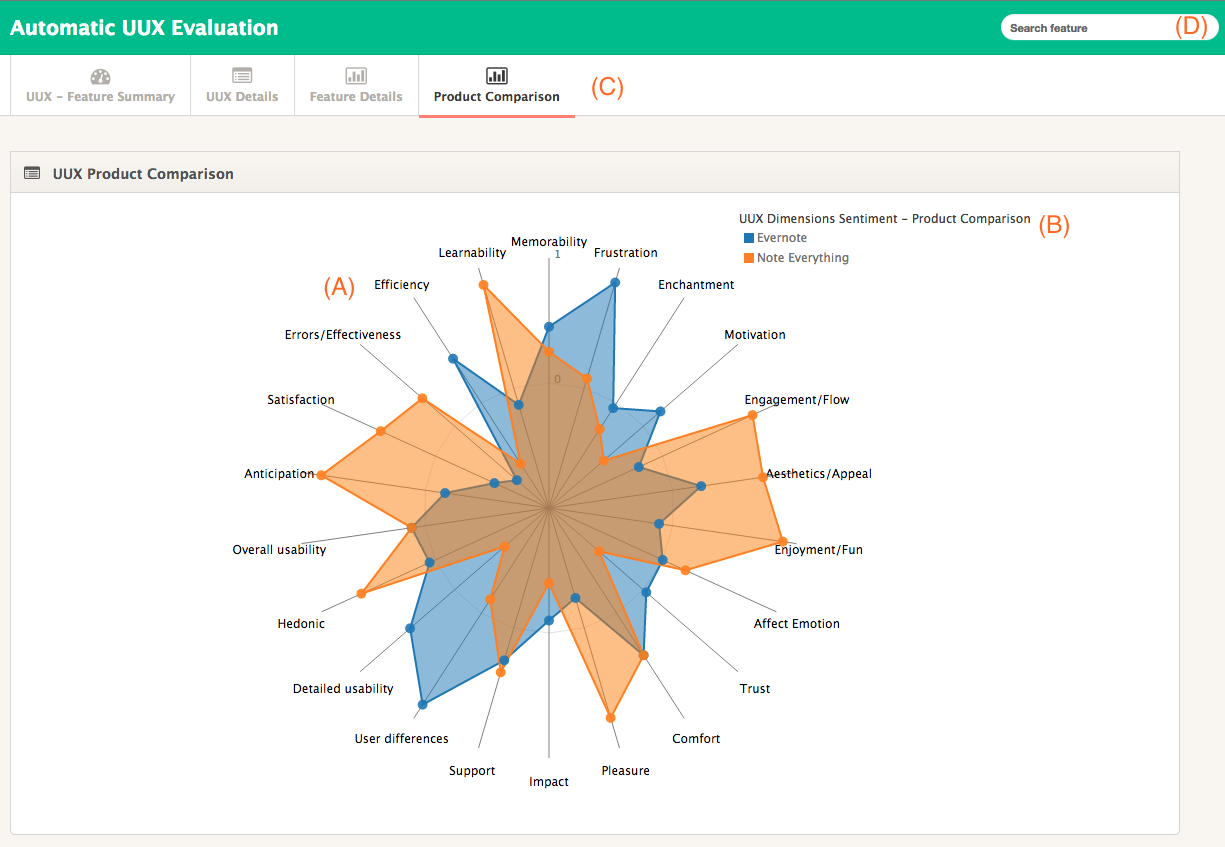
\includegraphics[width=0.4\textwidth]{img/introduction_scenario3.png}
			\caption{Product Comparison. The following information is depicted in the view: (A) Average sentiment of each UUX dimension for each of the products being compared, (B) General information (name, corresponding chart color) of the products, (C) Navigation menu, (D) Search field to query features.}
			\label{fig:introduction_scenario3}
		\end{figure}
      
         

\section{Evaluation Method}
\label{sec:Evaluation}
TODOS
We would probably have a section for each of the steps in the approach. 
Need to define ONE dataset for the whole project
Pending: Evaluation for the visualization, probably we could do a subject evaluation with 12 subjects...

\section{Evaluation Results} 
\label{sec:results}
\input{results}


%\section{Discussion}
%\label{sec:discussion}
%In this section we discuss the obtained results

\section{Discussion}
\label{sec:threats}
\input{discussion}

\section{Related Work}
\label{sec:related}
\subsection{Mining App Store Reviews}

Harman \etal \cite{paper:Harman} introduced app store mining and analyzed technical and business aspects of apps by extracting app features from the official app descriptions. 

Chandy and Gu \cite{paper:Chandy} classified spam in the AppStore through a latent model capable of classifying apps, developers, reviews and users into the normal and malicious categories. 

Pagano and Maalej \cite{paper:Pagano} investigated the types of user feedback present in the reviews and applied frequent item set mining for identifying feedback type patterns in user reviews, we map some of their findings into the labels we used in this work. 

Iacob and Harrison \cite{paper:Iacob} extracted feature requests from app store reviews by means of linguistic rules and used Latent Dirichlet Allocation (LDA) \cite{paper:Blei2003} to group the feature requests. In contrast with this work, we employed linguistic rules, text analysis, and sentiment analysis to mine different information from user reviews (not only feature requests).  
LDA was also used for: (i) feature based sentiment analysis of reviews\cite{paper:Guzman}, (ii) user reviews summarization\cite{paper:Galvis}, and (iii) the identification of incorrectly rated reviews\cite{paper:Fu}. 
%Guzman and Maalej\cite{paper:Guzman} extracted app features through a collocation and LDA algorithm. They assigned each %feature a sentiment through sentiment analysis. %Our work could be complemented with this existing work so that the extracted %features are associated to a specific software maintenance cateogry. 
%Galvis Carre\~no and Winbladh \cite{paper:Galvis} applied LDA to summarize user reviews. Our approach could use the topics %generated by LDA to group semantically similar reviews which belong to the same category. 
%Fu \etal \cite{paper:Fu} analyze user reviews from Google Play and apply a linear regression model combining the text from the %reviews and its ratings to identify incorrectly rated reviews. They input the words classified as negative words into an LDA %algorithm to find the main reason why users are unsatisfied with the app. 

Chen \etal \cite{paper:ARminer} used Naive Bayes for finding informative review sentences and LDA for grouping sentences with similar content. They then rank the groups of reviews according to a scheme which analyzes volume, time patterns and ratings. In our evaluation we filtered non-informative reviews using Chen's \etal approach. Similarly to Chen \etal \cite{paper:ARminer} we could rank the sentences that are considered more important in each of the software maintenance and evolution categories. 

Li \etal \cite{paper:Li} analyze user reviews to measure user satisfaction by matching words or phrases in the user comments with a predefined dictionary. 

\subsection{Classifying Reviews in UUX Dimensions} 



\section{Conclusions and Future Work}
\label{sec:conclusion}
\input{conclusions}

% use section* for acknowledgement
%\section*{Acknowledgment}
%The authors would like to thank...


% trigger a \newpage just before the given reference
% number - used to balance the columns on the last page
% adjust value as needed - may need to be readjusted if
% the document is modified later
%\IEEEtriggeratref{8}
% The "triggered" command can be changed if desired:
%\IEEEtriggercmd{\enlargethispage{-5in}}
 
% references section

% can use a bibliography generated by BibTeX as a .bbl file
% BibTeX documentation can be easily obtained at:
% http://www.ctan.org/tex-archive/biblio/bibtex/contrib/doc/
% The IEEEtran BibTeX style support page is at:
% http://www.michaelshell.org/tex/ieeetran/bibtex/
%\bibliographystyle{IEEEtran}
% argument is your BibTeX string definitions and bibliography database(s)
%\bibliography{IEEEabrv,../bib/paper}
%
% <OR> manually copy in the resultant .bbl file
% set second argument of \begin to the number of references
% (used to reserve space for the reference number labels box)
%\begin{thebibliography}{1}

%\end{thebibliography}
%\balance
%\bibliographystyle{IEEEtran}
%\bibliography{paper}  
     
     
\begin{thebibliography}{1}

\bibitem{paper:AntoniolICSME2008}
G.~Antoniol, K.~Ayari, M.~Di Penta, F.~Khomh, Y.~Guhneuc, \emph{Is it a bug or an enhancement?: a text-based approach to classify change requests}. CASCON, 2008:23.

\bibitem{paper:Bacchelli}
A. Bacchelli, T. Dal Sasso, M. D'Ambros, and M. Lanza. \emph{Content classification of development emails}. In Proceedings of the 34th International Conference on Software Engineering (ICSE), 2012, pp. 375-385. 

\bibitem{paper:Basili1996}
V. R.~Basili, L. C.~Briand, and W. L.~Melo, \emph{A validation of object oriented design metrics as quality indicators,} IEEE Trans. Software Eng., vol. 22, no. 10, pp. 751-761, 1996. 

\bibitem{paper:Bezerra2007}
M. Bezerra, A. L. I. Oliveira, and S. R. L. Meira, , \emph{A constructive rbf neural network for estimating the probability of defects in software modules,} in Neural Networks, 2007. IJCNN 2007. International Joint Conference on, 2007, pp. 2869-2874. 

\bibitem{paper:Blei2003}
D. M. ~Blei, A.Y. ~Ng, and M. I. ~Jordan, \emph{Latent dirichlet allocation}, in Journal of Machine Learning Research (JMLR), Vol. 3, 2003, pp. 993-1022.

\bibitem{paper:Cer2010}
D. Cer, M.C. de Marneffe, D. Jurafsky, and C.D. Manning, \emph{Parsing to Stanford dependencies: Trade-offs between speed and accuracy}, in Proceedings of the 7th International Conference on Language Resources and Evolution (LREC), 2010.

\bibitem{paper:Ceylan2006}
E. Ceylan, F. Kutlubay, and A. Bener, , \emph{Software defect identification using machine learning techniques,} in Software Engineering and Advanced Applications, 2006. SEAA ?06. 32nd EUROMICRO Conference on, 2006, pp. 240-247. 

\bibitem{paper:Chandy}
R. Chandy and H. Gu. \emph{Identifying spam in the iOS app store}. In Proceedings of the 2nd Joint WICOW/AIRWeb Workshop on Web Quality (WebQuality), 2012, pages 56-59.

\bibitem{paper:ARminer}
N.~Chen, J.~Lin, S.C.H.~Hoi, X.~Xiao, B.~Zhang, \emph{AR-miner: mining informative reviews for developers from mobile app marketplace}. In Proceedings of the 36th International Conference on Software Engineering (ICSE), 2014, pp. 767-778. 

\bibitem{paper:Chhetri2014}
Y. B. Chhetri and M. P. Robillard, \emph{Recommending Reference API Documentation}, in Empirical Software Engineering, 2014. To appear

\bibitem{paper:Dagan2005}
I. Dagan, O. Glickman, and B. Magnini,  \emph{The PASCAL recognizing textual entailment challenge}, in Proceedings of The First International Conference on Machine Learning Challenges: evaluating Predictive Uncertainly Visual Object Classification, and Recognizing Textual Entailment, 2005, pp. 177-190.

\bibitem{paper:deMarneffe2008}
M.C. de Marneffe, B. MacCartney, and C.D. Manning, , \emph{Generating typed dependency parses from phrase structure parses}, in Proceedings of LREC, 2006, pp. 449-454.

\bibitem{paper:Demsar2006}
J. Dem{\v s}ar,  \emph{Statistical comparisons of classifiers over multiple data sets}, in Journal of Machine Learning Research v.7, 2006, pp. 1-30.

\bibitem{paper:IR1992}
W. B.~Frakes and R.~Baeza-Yates, \emph{Information Retrieval: Data Structures and Algorithms?}. Prentice-Hall, Englewood Cliffs, NJ, 1992.

\bibitem{paper:Fu}
B. Fu, J. Lin, L. Li, C. Faloutsos, J. Hong, and N. Sadeh. \emph{Why people hate your app: Making sense of user feedback in a mobile app store.}. In Proc. of the International Conference on Knowledge Discovery and Data Mining (KDD), 2013, pages 1276-1284.

\bibitem{paper:Fundel2007}
K. Fundel, R. K\'"uffner, and R. Zimmer, \emph{RelEx - Relation extraction using dependency parse trees}, in Bioinformatics, v.23, n.3, 2007, pp. 365-371.

\bibitem{paper:Galvis}
L. V. Galvis Carreño and K. Winbladh. \emph{Analysis of user comments: an approach for software requirements evolution}. In Proceedings of the 2013 International Conference on Software Engineering (ICSE), 2013, pages 582-591. 

\bibitem{paper:Guzman}
E. ~Guzman, and W. ~Maalej \emph{How Do Users Like This Feature? A Fine Grained Sentiment Analysis of App Reviews}. In Proceedings of the 22nd IEEE International  Requirements Engineering Conference (RE), 2014, pp. 153-162

\bibitem{paper:Guzzi2013}
A. Guzzi, A. Bacchelli, M. Lanza, M. Pinzger, and A. van Deursen, 
\emph{Communication in open source software development mailing lists},
in Proceedings of the 10th Working Conference on Mining Software Repositories 
(MSR), 2013, pp 277-286. 

\bibitem{paper:Guzzi2012}
A. Guzzi, A. Begel, J.K. Miller, and K. Nareddy, 
\emph{Facilitating Enterprise Software Developer Communication with CARES},
in Proceedings of the 34th International Conference on Software Engineering 
(ICSE), 2012, pp 1367-1370. 

\bibitem{paper:Harman}
M. Harman, Y. Jia, and Y. Zhang. \emph{App store mining and analysis: MSR for app stores.} In Proc. of the Working Conference on Mining Software Repositories (MSR) 2012, pages 108-111.

\bibitem{paper:Iacob}
C. Iacob and R. Harrison. \emph{Retrieving and analyzing mobile apps feature requests from online reviews}. In Proc. of the Working Conference on Mining Software Repositories (MSR), 2013, pages 41-44.

\bibitem{paper:Kucuktunc}
O. Kucuktunc, B. B. Cambazoglu, I. Weber, and H. Ferhatosmanoglu. \emph{A large-scale sentiment analysis for Yahoo! Answers}, In Proceedings of the International Conference on Web Search and Data Mining (WSDM), 2012, pp 633-642.

\bibitem{paper:Li}
H. Li, L. Zhang, L. Zhang, and J. Shen. \emph{A user satisfaction analysis approach for software evolution}. In Proc. of the Progress in Informatics and Computing Conference (PIC), 2010, volume 2, pages 1093-1097.

\bibitem{paper:Liu2010}
Y. Liu, T. M. Khoshgoftaar, and N. Seliya, , \emph{Evolutionary optimization of software quality modeling with multiple repositories,} IEEE Trans. Softw. Eng., vol. 36, no. 6, Nov. 2010, pp. 852-864. 

\bibitem{paper:Nivre2010}
J. Nivre, L. Rimell, R. McDonald, and C. G\'omez-Rodr\'iguez, \emph{Evaluation of dependency parsers on unbounded dependencies}, in Proceedings of COLING, 2010, pp. 813-821.

\bibitem{paper:Pagano}
D.~Pagano, and W.~Maalej \emph{User Feedback in the AppStore: An Empirical Study}. In Proceedings of the 21st IEEE International Requirements Engineering Conference (RE), 2013, pp.125-134.

\bibitem{paper:Pandita2012}
R. Pandita, X.Xiao, H. Zhong, and T. Xie, \emph{Inferring method specifications from natural language API descriptions}, in Proceedings of the 34th International Conference on Software Engineering (ICSE), 2012, pp. 815-825

\bibitem{paper:Pang}
B. Pang, L. Lee,  and S. Vaithyanathan,  \emph{Thumbs up?: sentiment classification using machine learning techniques}, Proceedings of the ACL-02 Conference on Empirical Methods in Natural Language Processing, pp. 79-86, 2002.

\bibitem{paper:Panichella2012}
S. Panichella, J. Aponte, M. Di Penta, A. Marcus, and G. Canfora \emph{Mining source code descriptions from developers communications}, in Proceedings of the 20th IEEE International Conference on Program Comprehension, 2012, pp. 63-72.

\bibitem{paper:Slankas2014}
J. Slankas, X. Xiao, L. Williams, and T. Xie, \emph{Relation extraction for inferring access control rules from natural language artifacts}, in Proceedings of the 30th Annual Computer Security Applications Conference (ACSAC), 2014, pp. 366-375.

\bibitem{paper:ML2005}
I.~Witten and E.~Frank, \emph{Data Mining: Practical Machine Learning Tools and Techniques}. Morgan Kaufmann, 2005. 

\bibitem{paper:ZhouText2014} 
Y. ~Zhou, Y.~Tong, R.~Gu, H.~Gall, \emph{Combining Text Mining and Data Mining for Bug Report Classification?}. In Proceeding of 30th International Conference on Software Maintenance and Evolution (ICSME), 2014, pp. 311-320.

\bibitem{paper:Zimmermannesem2009}
T. Zimmermann and N. Nagappan, , \emph{Predicting defects with program dependencies}, in Empirical Software Engineering and Measurement, 2009. ESEM 2009. 3rd International Symposium on, 2009, pp. 435-438. 


%\bibitem{paper:Kaur}
%A. ~Kaur, Er. ~Nidhi Gumber \emph{A Review on Sentimental Analysis of Application %Reviews}. In International Journal of Modern Engineering Research (IJMER), Vol 4, Iss. 6, %June 2014. pp. 72-76.
 
%\bibitem{paper:Sentiwordnet}
%A. ~Esuli, and F. ~Sebastiani \emph{SentiWordNet: A publicly available lexical resource for opinion mining}. In Proceedings of %Language Resources and Evaluation Confernce (LREC), 2006, pp. 417-422.

%\bibitem{paper:Hamouda}
%A.~Hamouda, and A.~Rohaim \emph{Reviews Classification Using SentiWordNet Lexicon}. in Journal on Computer Science and %Information Technology (OJCSIT), Vol. (2), No.(1), 2011. 


\end{thebibliography}
		    
\end{document}







